\documentclass[a4paper, 12pt]{article}

\usepackage[portuges]{babel}
\usepackage[utf8]{inputenc}
\usepackage{amsmath}
\usepackage{indentfirst}
\usepackage{blindtext}
\usepackage{graphicx}
\usepackage[hidelinks]{hyperref}
\usepackage{gensymb}
\usepackage{pgfplots}

\author{Igor Abreu da Silva}

\title{Trabalho Final de Sistemas Lineares I}

\begin{document}

    \begin{titlepage}
        \begin{center}
            \huge{Universidade Federal do Rio de Janeiro}
            \vspace{95pt}

            \large{Lista IV - Sistemas Lineares I}
            \vspace{160pt}
        \end{center}

        \begin{flushleft}
            \begin{tabbing}
                Alunos\qquad\qquad\= Igor Abreu da Silva\\
                DRE\> 112053874 \\
                Curso\> Engenharia Eletrônica \\
                Turma\> 2016/2 \\
                Professor\> Natanael Nunes de Moura Junior \\

            \end{tabbing}

        \end{flushleft}

        \begin{center}
            \vspace{\fill}
            Rio de Janeiro, 16 de Novembro de 2016
        \end{center}
    \end{titlepage}

    \newpage
    \tableofcontents
    \listoffigures
    \thispagestyle{empty}
    \newpage
    \pagenumbering{arabic}

\section{Diagrama de P\'{o}los e Zeros}
    \subsection{Quest\~{a}o 1}
        \subsubsection{Item a}
        \[\frac{1}{s+1} + \frac{1}{s+3} = \frac{(s+3) + (s+1)}{(s+1)(s+3)} = \frac{2s + 4}{s^{2} + 4s + 4}\]\\
        \[Zeros: 2s + 4 = 0 \rightarrow s = -2\]
        \[Polos:  s^{2} + 4s + 4 = 0 \rightarrow s = -2\]
		\begin{figure}[!ht]
			\centering
			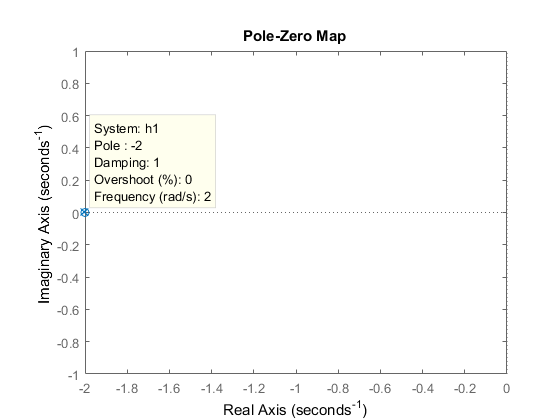
\includegraphics[scale=0.7]{img/Q1a.png}
			\caption{P\'{o}los e Zeros - Item a}	
		\end{figure}	        
		\newpage
        \subsubsection{Item b}
		\begin{figure}[!ht]
			\centering
			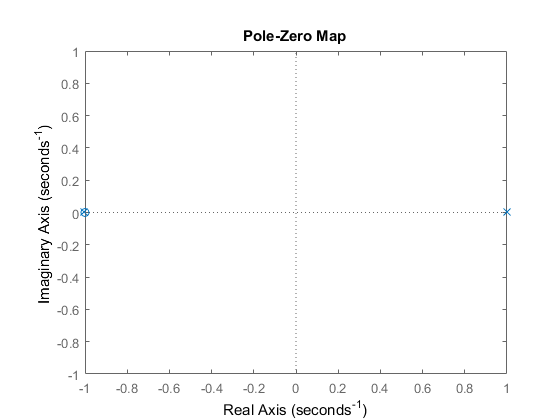
\includegraphics[scale=0.7]{img/Q1b.png}
			\caption{P\'{o}los e Zeros - Item b}	
		\end{figure}	   
		
        \[Zeros: s + 1 = 0 \rightarrow s = -1\]
        \[Polos:  s^{2} + 1 = 0 \rightarrow s = {-1; +1}\]
        \newpage
        \subsubsection{Item c}
		\begin{figure}[!ht]
			\centering
			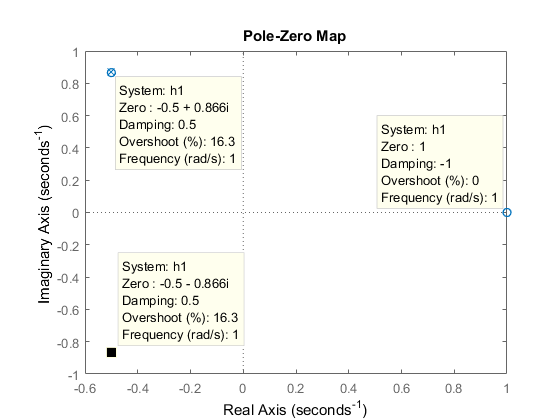
\includegraphics[scale=0.7]{img/Q1c.png}
			\caption{P\'{o}los e Zeros - Item c}	
		\end{figure}	   
		
		\[Zeros: s^{3} - 1 = 0 \rightarrow s = {\frac{-1 + \sqrt{3}}{2}; \frac{-1 - \sqrt{3}}{2}; 1}\]
		\[Polos:  s^{2} + s + 1 = 0 \rightarrow s = {\frac{-1 + \sqrt{3}}{2}; \frac{-1 - \sqrt{3}}{2}}\]        
\section{Propriedade da Transformada de Laplace}
    \subsection{Quest\~{a}o 2}
        \subsubsection{Item a}
			\[\int_{-\infty}^{+\infty} x(t-1)e^{-st}u(t)dt \rightarrow \int_{0}^{+\infty}x(\tau)e^{-s(\tau + 1)}d\tau \rightarrow e^{-s}\int_{0}^{+\infty}x(\tau)e^{-s\tau}d\tau\ \Rightarrow e^{-s}X(s)\]
        \subsubsection{Item b}
        Pela propriedade da derivação de Laplace, temos:
        \[s^3X{s} - s^2x(0^{-}) + sx^{'}(0^{-}) - x^{''}(0^{-})\]
        \newpage
        \subsubsection{Item c}
        Pela propriedade da integração de Laplace, temos:
        \[\frac{X(s)}{s}\]
    \subsection{Quest\~{a}o 3}
    \[\int_{-\infty}^{+\infty} cos(\omega_{0}t)u(t)e^{-st}dt \rightarrow = \frac{1}{2}\int_{0}^{\infty} e^{-t(s-\omega _{0})} + e^{-t(s+\omega _{0})}dt \rightarrow \]
    \[\frac{1}{2(s-w_{0})} + \frac{1}{2(s+w_{0})} \rightarrow \frac{s}{s^{2} + \omega _{0}^{2} } \]
\section{Resposta em Frequ\^{e}ncia}
    \subsection{Quest\~{a}o 4}
        \subsubsection{Item a}
        \subsubsection{Item b}
        \subsubsection{Item c}
    \subsection{Quest\~{a}o 5}
        \subsubsection{Item a}
        \subsubsection{Item b}
        \subsubsection{Item c}
        \subsubsection{Item d}
        \subsubsection{Item e}
    \subsection{Quest\~{a}o 6}
        \subsubsection{Item a}
        É possível, uma vez que a resposta e um deslocamento de fase.
        \subsubsection{Item b}
        Não é possível, uma vez que ocorre uma alteração na frequência.
        \subsubsection{Item c}
        É possível, o sinal de saída e o mesmo que a entrada.
\section{Diagrama de Bode}
    \subsection{Quest\~{a}o 7}
        \subsubsection{Item a}
        \subsubsection{Item b}
        \subsubsection{Item c}
        \subsubsection{Item d}
    \subsection{Quest\~{a}o 8}
        \subsubsection{Item a}
        \subsubsection{Item b}
        \subsubsection{Item c}
        \subsubsection{Item d}
\end{document}